	\begin{frame}{Nền tảng Học tăng cường}
		\begin{columns}
		\column{0.6 \textwidth}
        \begin{itemize}
    		\begin{block}{Khái quát học tăng cường (Reinforcement Learning)}
    		    \begin{itemize}
    		    \setlength\itemsep{0.01em}
    		    \item Một kiểu học máy chính bên cạnh học có giám sát và học không giám sát.
    		    \item 2 đối tượng chính: tác nhân - \emph{Agent} và môi trường - \emph{Environment}.
    		    \item Mục tiêu: Tác nhân thu được tổng phần thưởng lớn nhất khi tương tác với mối trường qua các hành động.
    		    \end{itemize}
    		    \textcolor{blue}{Thành phần chính}:
    		    \begin{itemize}
    		        \setlength\itemsep{0.01em}
        		    \item \textbf{policy function}: Ánh xạ từ tập trạng thái của môi trường đến tập hành động.
        		    \item \textbf{reward}: Phần thưởng qua mỗi hành động của tác nhân.
        		    \item \textbf{value function}: Tổng phần thưởng dự kiến của agent.
    		    \end{itemize}
    		\end{block}
		\end{itemize}
		\column{0.4 \textwidth}
		\begin{figure}[ht]
            \fbox{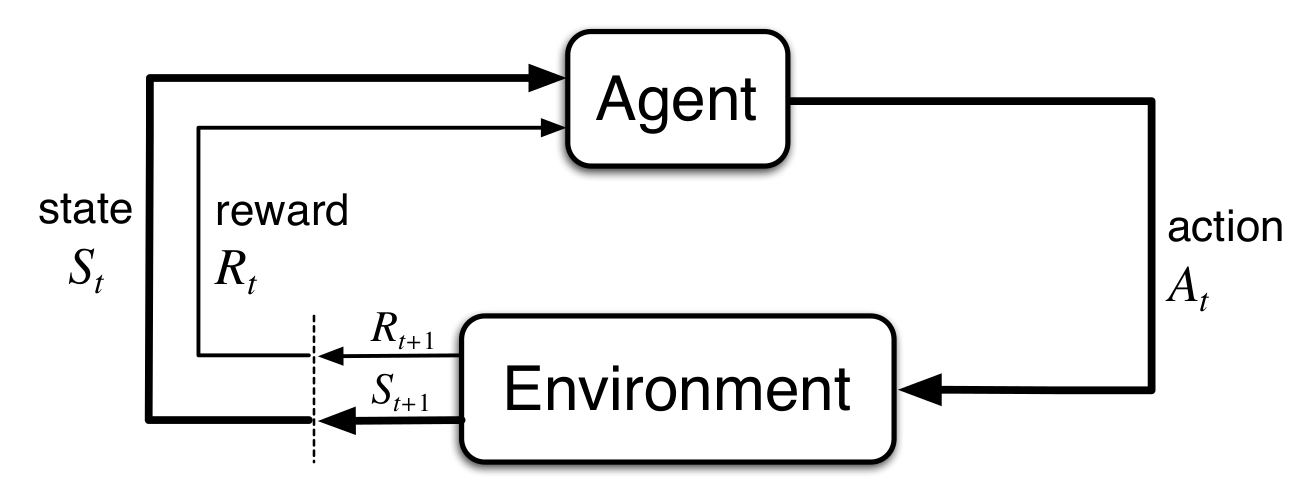
\includegraphics[width=0.9\linewidth]{images/mdp.png}}
            \caption{Chu trình học trong học tăng cường. Quá trình quyết định Markov}
            \label{fig:problem:mdp}
        \end{figure}
		\end{columns}
	\end{frame}
	\begin{frame}{Huấn luyện mô hình học tăng cường}
		\begin{columns}
		\column{0.6 \textwidth}
        \begin{itemize}
    		\begin{block}{Phương pháp}
    		    \begin{itemize}
    		    \setlength\itemsep{0.01em}
    		    \item Sử dụng \emph{tabular methods}. Chỉ phù hợp với mô hình đơn giản.
    		    \item Tối ưu hóa hàm mục tiêu \emph{policy function}, \emph{value function}
    		    \end{itemize}
    		\end{block}
    		\begin{block}{Tối ưu hóa \emph{policy function} sử dụng mạng Nơ-ron}
    		    \begin{itemize}
    		    \setlength\itemsep{0.01em}
    		    \item Coi \emph{policy function} là một mạng nơ-ron.
    		    \item Đầu vào của mạng là trạng thái của \emph{environment}. Đầu ra của mạng là \emph{action} của \emph{agent}.
    		    \item Phần thưởng thu được chính là độ đo để đánh giá chất lượng của mô hình mạng.
    		    \end{itemize}
    		\end{block}
		\end{itemize}
		\column{0.4 \textwidth}
		\begin{figure}[ht]
            \centering
            \fbox{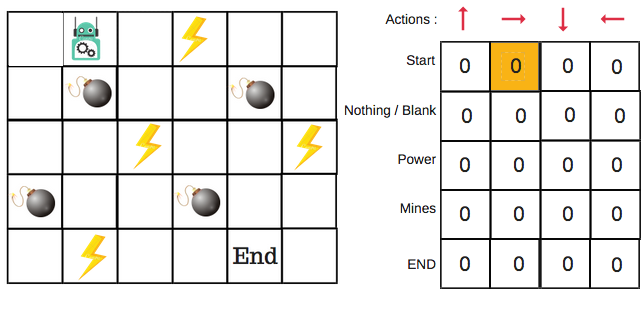
\includegraphics[width=0.9\linewidth]{images/tabular-table.png}}
            \caption{Tabular Methods}
            \label{fig:problem:tabular}
            \fbox{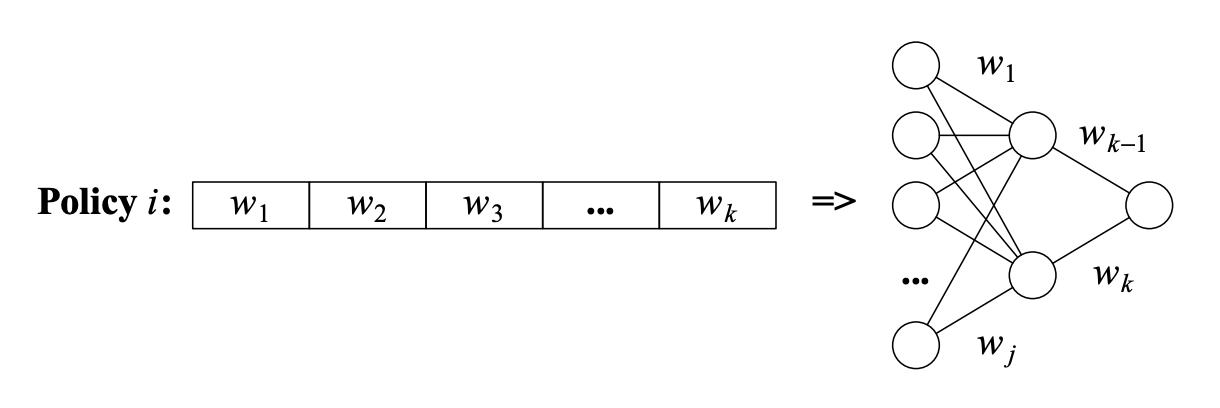
\includegraphics[width=0.9\linewidth]{images/policy.png}}
            \caption{Biểu diễn policy}
        \end{figure}
		\end{columns}
	\end{frame}
	
	\begin{frame}{Vấn đề khi huấn luyện policy function}
	    \begin{itemize}
	    \begin{block}{Vấn đề}
	    \textcolor{red}{Khi thông số môi trường thay đổi thì trạng thái cũng thay đổi theo. \emph{Policy} tối ưu vừa học không còn phù hợp, phải huấn luyện lại từ đầu.}
	    \end{block}
	    \begin{block}{Phát biểu bài toán}
	        \begin{itemize}
    		    \setlength\itemsep{0.01em}
    		    \item Cho $K$ tác vụ $T_1, T_2, ..., T_K$.
    		    \item Giả sử $h_k$ là bộ tham số môi trường tương ứng với tác vụ $T_k$, $h_j$ là bộ tham số môi trường tương ứng với tác vụ $T_j$ và $h_j \neq h_k$.
    		    \end{itemize}
    		    Mục tiêu: 
    		    \begin{itemize}
    		        \item Mỗi tác vụ được biểu diễn bởi một mạng Nơ-ron.
    		        \item Khai thác mối quan hệ tiềm ẩn, tối ưu hóa đồng thời $K$ tác vụ.
    		    \end{itemize}
	    \end{block}
	    \end{itemize}
	\end{frame}
	
	\begin{frame}{Tối ưu hóa đa nhiệm nhiều mạng policy}
	    \begin{itemize}
    	    \begin{block}{Giả định}
    	    \begin{itemize}
    	        \item Mỗi tác vụ là một nhiệm vụ tối ưu \emph{policy}, tương đương với việc tối ưu một mạng nơ-ron.
    	        \item Các mạng nơ-ron có cùng cấu trúc.
    	        \item Bộ dữ liệu đầu vào của mỗi mạng là tương đối khác nhau do thay đổi tham số môi trường.
    	    \end{itemize}
    	    \end{block}
    	    \begin{block}{Giải quyết}
    	    \begin{itemize}
    	        \item Áp dụng mô hình thuật toán tối ưu hóa đa nhiệm.
    	        \item Mỗi cá thể được mã hóa, giải mã bằng phương pháp mã hóa, giải mã đề xuất.
    	        \item Hàm đánh giá là tổng phần thưởng \emph{agent} nhận với mô hình policy trong tác vụ tương ứng
    	    \end{itemize}
    	    \end{block}
	    \end{itemize}
	\end{frame}
	
	\begin{frame}{Phương pháp tiến hóa đề xuất tối ưu policy function}
		\begin{columns}
		\column{0.5 \textwidth}
        \begin{itemize}
    		\begin{block}{Mã hóa và giải mã nhiễm sắc thể}
    		    \begin{itemize}
    		    \setlength\itemsep{0.01em}
    		    \item Các tham số trong mạng lần lượt được mã hóa "trực tiếp" vào nhiễm sắc thể.
    		    \item Quá trình giải mã ngược lại để đánh giá mô hình mạng.
    		    \end{itemize}
    		\end{block}
    		\begin{block}{Áp dụng EA để huấn luyện mạng}
    		    \begin{itemize}
    		    \setlength\itemsep{0.01em}
    		    \item \emph{fitness} của cá thể là tổng phần thưởng thu được từ mô hình hiện tại.
    		    \item Mô hình policy càng tối ưu thì tổng phần thưởng thu được càng cao.
    		    \end{itemize}
    		\end{block}
		\end{itemize}
		\column{0.48 \textwidth}
		\begin{figure}[ht]
            \centering
            \fbox{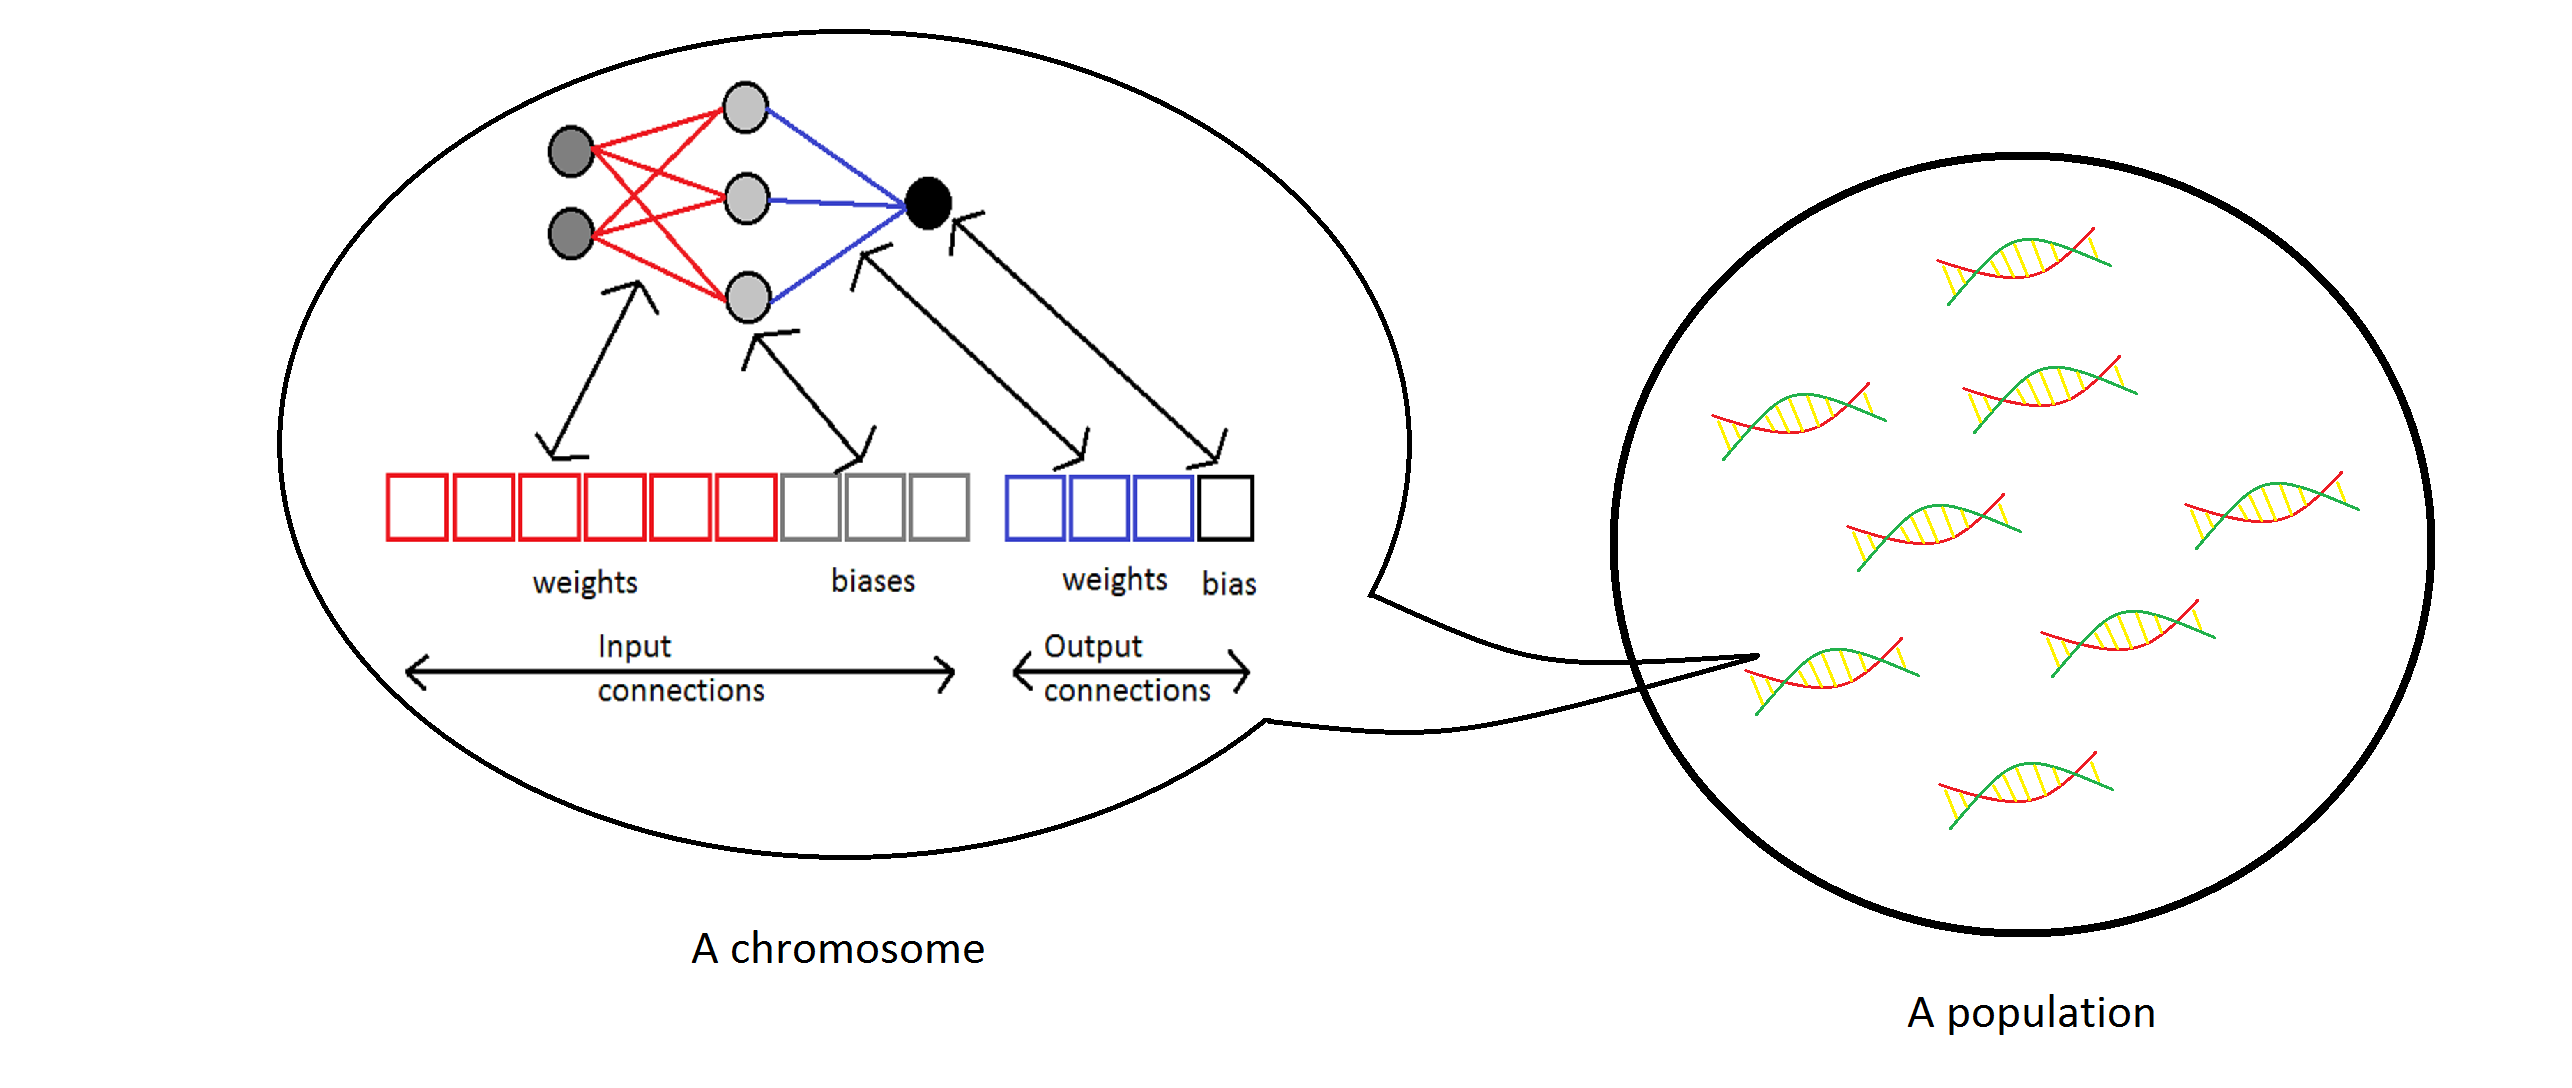
\includegraphics[width=0.95\linewidth]{images/proposed_encoding.png}}
            \caption{Mã hóa và giải mã policy.}
            \label{fig:problem:policy}
            \fbox{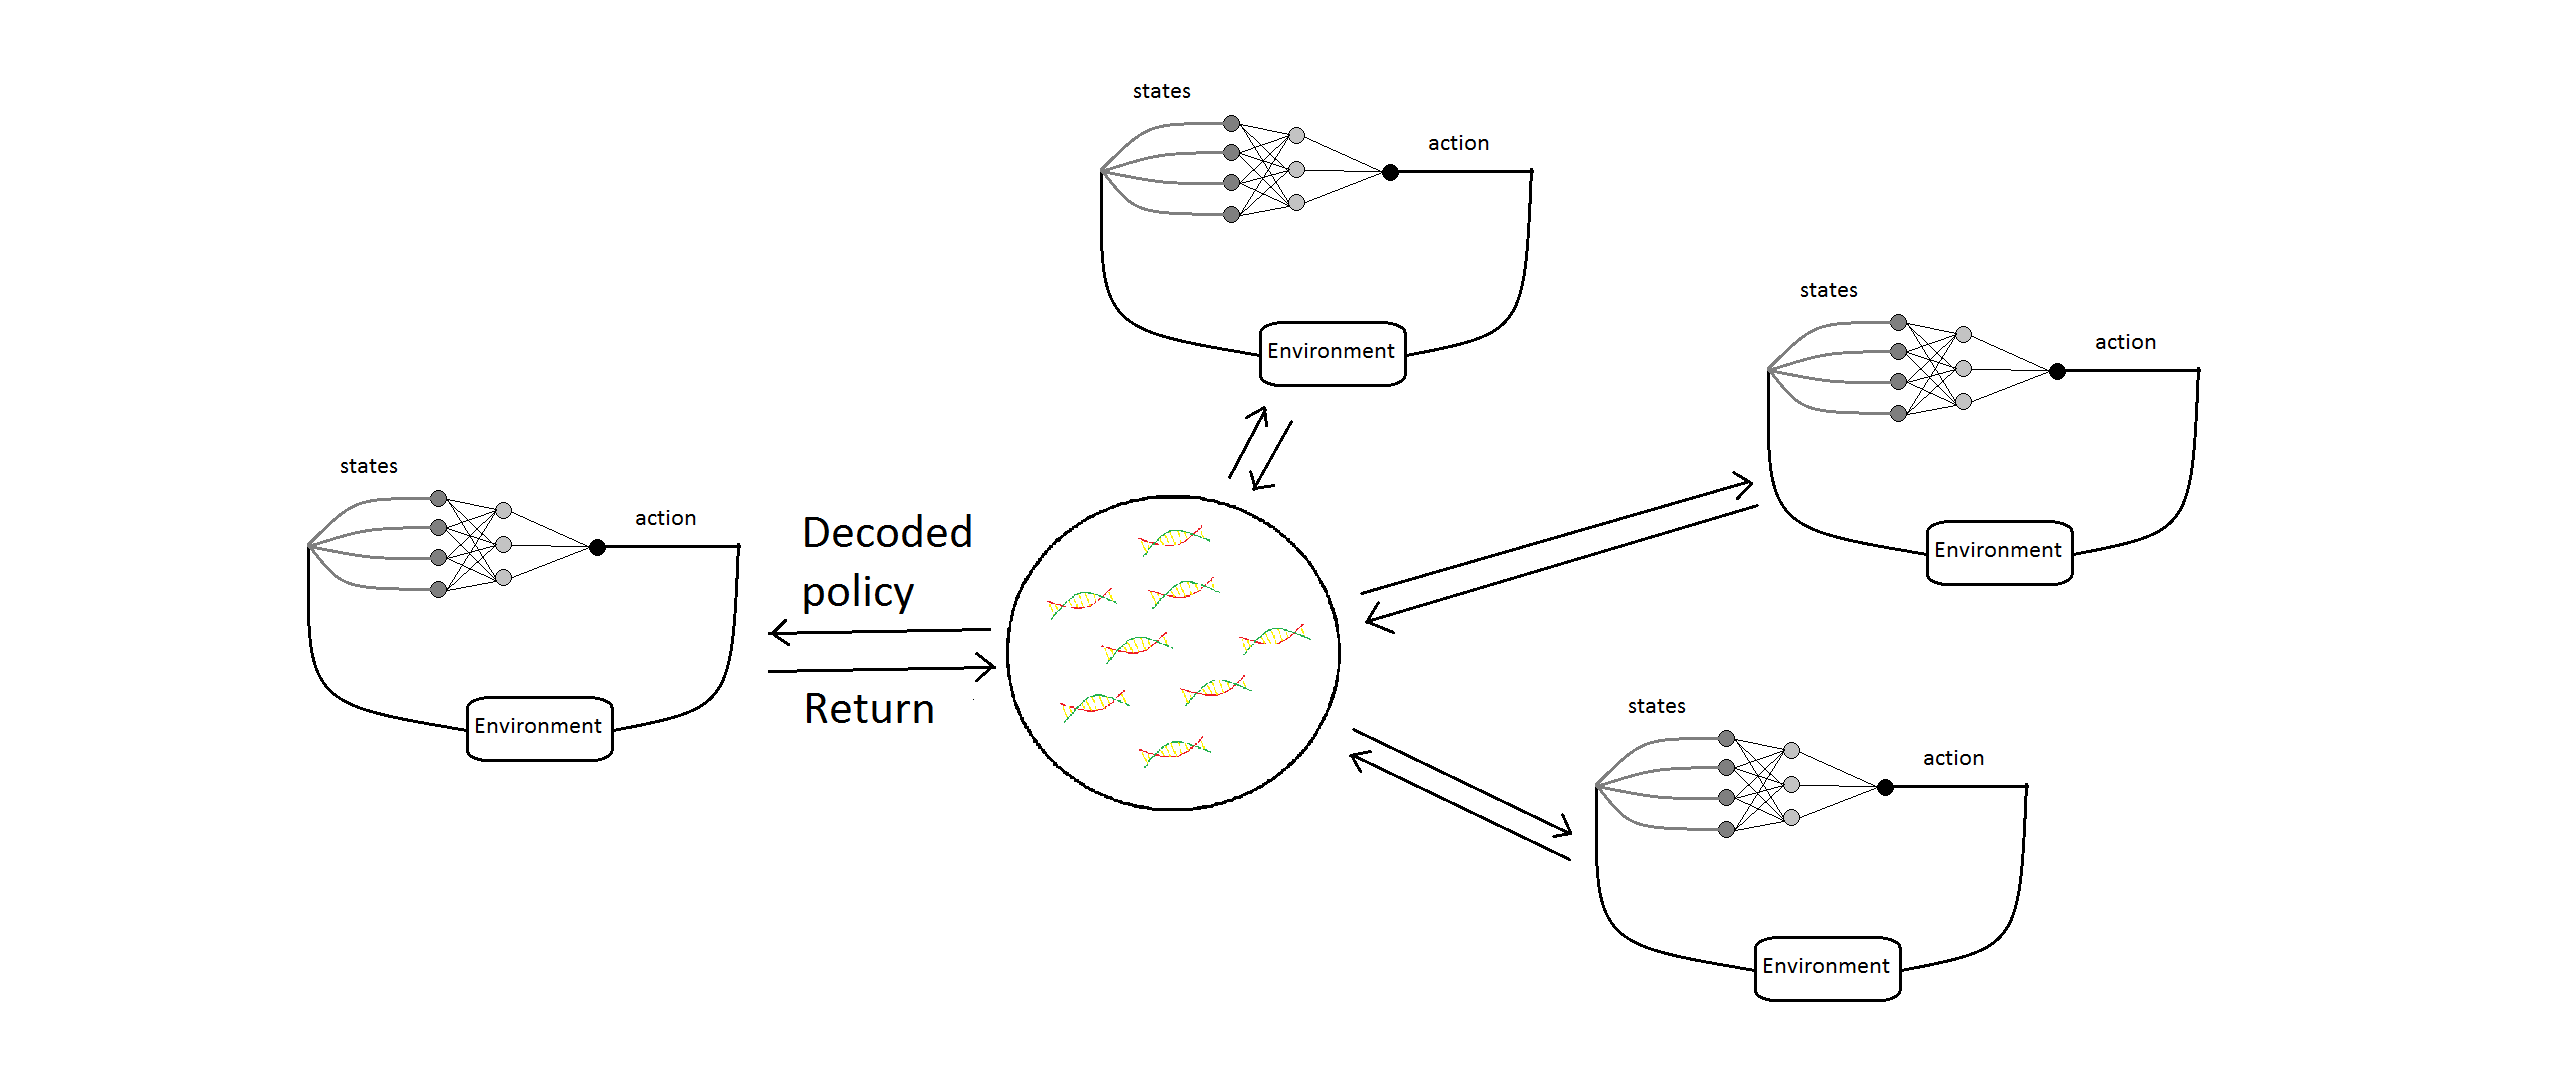
\includegraphics[width=0.95\linewidth]{images/proposed_ea.png}}
            \caption{Toàn cảnh dùng EA để tối ưu hóa policy}
        \end{figure}
		\end{columns}
	\end{frame}